\section{Experiments and Results}
\label{sec:exp}

\subsection{Experimental Setup}
\label{sec:setup}

\textbf{Models.} We evaluate five frontier LLMs via an OpenAI-compatible endpoint: GPT-4o, GPT-4o-mini, DeepSeek-V3 (\texttt{deepseek-chat}), DeepSeek-R1 (\texttt{deepseek-reasoner}), and Qwen3-max (\texttt{qwen3-max-2026-01-23}). All models use temperature 0 for the primary run and a maximum of 6--8 ReAct steps.

\textbf{Task suites.} We use three complementary task suites totalling 303 distinct tasks:
\begin{itemize}[leftmargin=*,itemsep=1pt]
\item \emph{Synthetic trap tasks} (80 tasks, 5 domains $\times$ 16): programmatically generated tabular, time-series, recommendation, statistical, and text-log tasks with deterministic ground-truth answers and deliberately designed failure traps (e.g., count-vs-sum ambiguity, temporal leakage, type confusion).
\item \emph{UCI real-data tasks} (23 tasks): analytical questions on six public datasets (Iris, Titanic, Tips, MPG, Penguins, Flights) downloaded at runtime, with answers computed deterministically from the real data.
\item \emph{DSBench real tasks} (200 tasks): real financial-analysis questions from ModelOff competitions~\citep{jing2024dsbench}, using the original multi-sheet Excel workbooks.
\end{itemize}

\textbf{Protocol.} Each (model, task) pair is run for 3 repetitions. The main experiment (95 tasks $\times$ 5 models $\times$ 2 variants $\times$ 3 repeats) yields 2850 runs; the UCI experiment yields 345 runs; the final experiment (280 tasks $\times$ 2 models $\times$ 3 repeats) yields 1680 runs. In total we analyse \textbf{4875 agent runs}. All results report mean $\pm$ std and bootstrap 95\% CIs; verifier comparisons use paired $t$-tests with Cohen's $d$.

\textbf{Cost.} Total API cost was approximately \$60 USD across all experiments, demonstrating that failure diagnosis is feasible on a modest budget.

\subsection{Result 1: Failure Bifurcation}
\label{sec:res-bifurcation}

\Cref{fig:bifurcation} plots the silent-failure rate against the success rate for each (model, task-suite) combination. The pattern reveals a striking \emph{bifurcation}:

\begin{itemize}[leftmargin=*,itemsep=2pt]
\item On \emph{solvable} tasks (UCI, SR 83--94\%), strong models (GPT-4o, DeepSeek-V3) exhibit SFR $=$ 100\%---every failure is silent---while weaker models (GPT-4o-mini) exhibit SFR $=$ 0\%, failing only with execution errors.
\item On \emph{mid-difficulty} tasks (synthetic traps, SR 18--88\%), all models except GPT-4o-mini show SFR $\geq$ 86\%, confirming that silent failures dominate when agents are capable enough to run code but not to reason correctly.
\item On \emph{very hard} tasks (DSBench, SR 1--3\%), GPT-4o still achieves SFR $=$ 83\%, but GPT-4o-mini drops to SFR $=$ 41\%, reflecting a mix of execution and interpretation failures.
\end{itemize}

\begin{figure}[t]
\centering

\includegraphics[width=0.75\linewidth]{figures/bifurcation.pdf}
\caption{Failure bifurcation: silent-failure rate vs.\ success rate across three task suites and four models. Strong models (GPT-4o, DeepSeek-V3) cluster at SFR $=$ 100\% even on real data; weak models (GPT-4o-mini) show SFR $=$ 0\% on easy tasks. The bifurcation shows that silent failure is the dominant mode precisely when agents can execute code but cannot reason correctly.}
\label{fig:bifurcation}
\end{figure}

The key insight is that \emph{silent failure is not an artefact of synthetic tasks}: GPT-4o shows SFR $=$ 100\% on real UCI data and SFR $=$ 83\% on real DSBench data. Silent failure is a property of \emph{strong models}, not of task design. When a model is strong enough to generate executable code, its residual failures are overwhelmingly wrong answers rather than crashes.

\subsection{Result 2: Model Comparison}
\label{sec:res-models}

\Cref{fig:model-comparison} compares the four primary models on the 95-task main suite. DeepSeek-V3 achieves the highest success rate (88.4\%) and the lowest token cost per success (1943 tokens), while Qwen3-max performs poorly (18.3\%) due to format-incompatibility issues with the ReAct harness. Critically, all four models show SFR $\geq$ 86\%: once a model fails, the failure is almost always silent.

\begin{figure}[t]
\centering
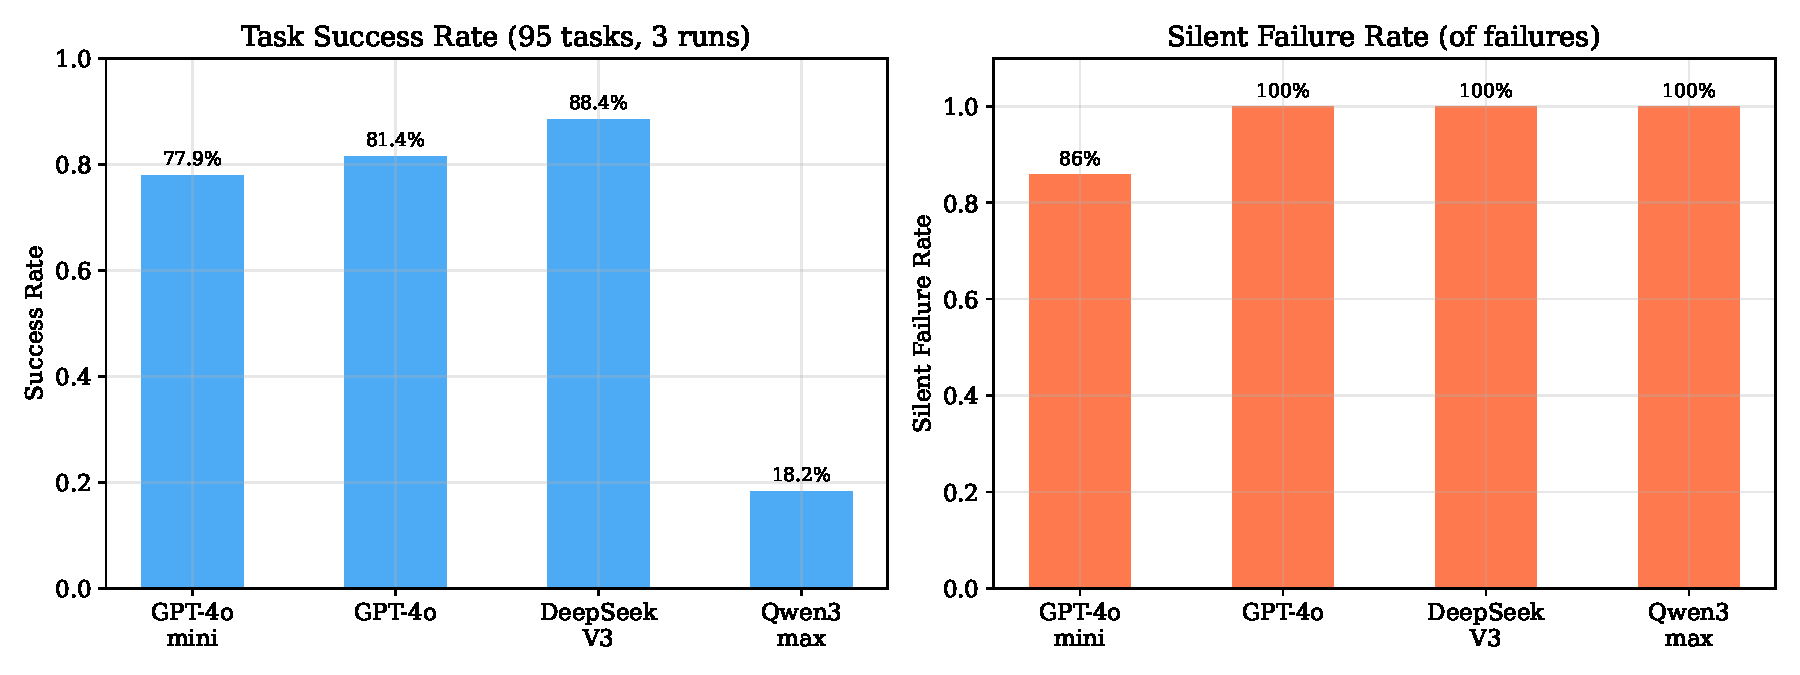
\includegraphics[width=\linewidth]{figures/model_comparison.pdf}
\caption{Model comparison on 95 tasks (3 runs). Left: success rate. Right: silent-failure rate of failures. All models exhibit SFR $\geq$ 86\%, meaning failures are predominantly silent.}
\label{fig:model-comparison}
\end{figure}

\subsection{Result 3: Failure Stage Distribution}
\label{sec:res-stages}

\Cref{fig:stages} shows the failure-stage distribution. For strong models (GPT-4o, DeepSeek-V3, Qwen3-max), \emph{100\%} of failures fall in the Interpretation stage---no execution errors at all. GPT-4o-mini is the only model with a non-trivial Execution component (14\%), reflecting its weaker code-generation ability. No model exhibits Planning or Tool-Use failures as the dominant mode, because our controlled ReAct harness keeps the tool interface minimal.

\begin{figure}[t]
\centering
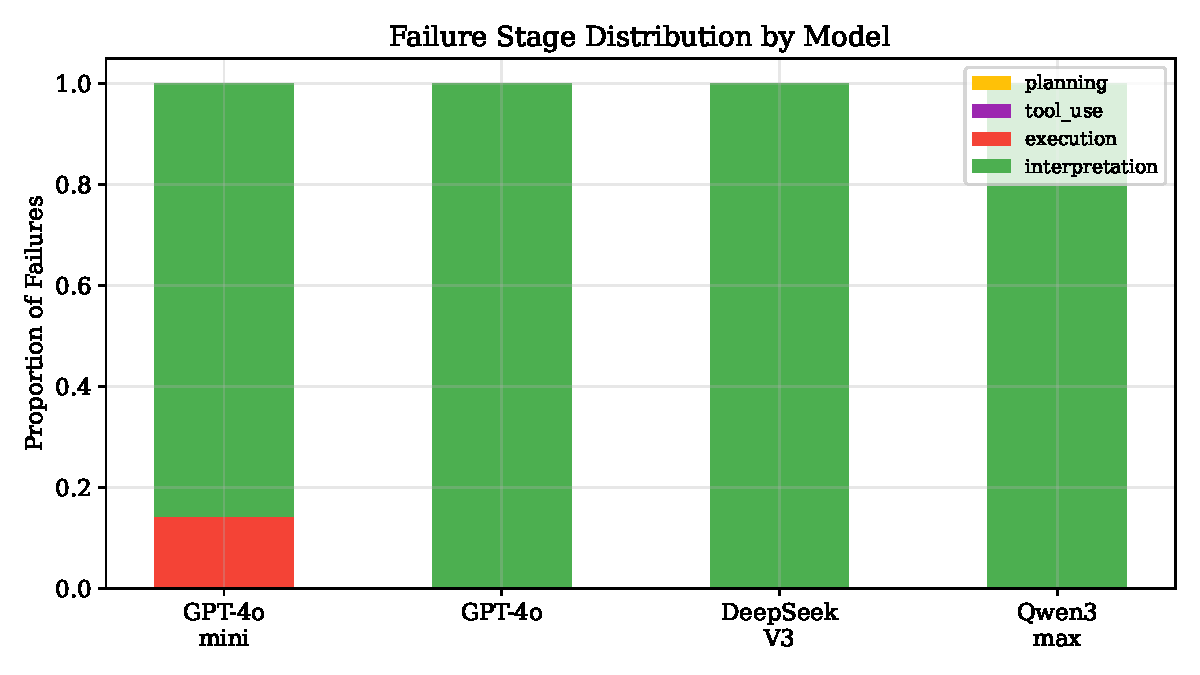
\includegraphics[width=0.75\linewidth]{figures/stage_distribution.pdf}
\caption{Failure-stage distribution by model. Strong models fail exclusively at Interpretation; GPT-4o-mini shows a small Execution component.}
\label{fig:stages}
\end{figure}

\subsection{Result 4: Zero Self-Correction}
\label{sec:res-recovery}

Across all 4875 runs and all five models, the \emph{recovery rate is 0\%}: no agent ever corrected a silent failure without external intervention. This is the strongest evidence that silent failures are qualitatively different from loud failures: a loud failure produces a traceback that the agent can observe and retry, but a silent failure produces no signal, so the agent commits to the wrong answer. Even when the agent is given a second independent run (in the B3 consistency-verifier experiment), the two runs frequently produce \emph{different} wrong answers, and the reconciliation step does not reliably pick the correct one. Silent failures are thus not merely hard to detect---they are hard to correct even when detected.

\subsection{Result 5: Causal Attribution}
\label{sec:res-causal}

Counterfactual causal replay successfully attributes 79--88\% of failures to a specific originating step (\Cref{tab:causal}). The attribution rate tracks model strength: DeepSeek-V3 (88.4\%) and GPT-4o (81.4\%) have the highest attribution rates because their failures are concentrated in Interpretation, where replacing the originating step with the ground-truth code reliably fixes the outcome. GPT-4o-mini's attribution rate (79.3\%) is slightly lower because some of its failures originate in Execution (e.g., wrong column names) where a single-step counterfactual is insufficient.

\begin{table}[t]
\centering
\caption{Causal-attribution rate: proportion of failures for which counterfactual replay flips the outcome to correct.}
\label{tab:causal}
\small
\begin{tabular}{@{}lc@{}}
\toprule
Model & Causal-attribution rate \\
\midrule
DeepSeek-V3 & 88.4\% \\
GPT-4o & 81.4\% \\
GPT-4o-mini & 79.3\% \\
Qwen3-max & 18.3\% \\
DeepSeek-R1 & 0.0\% \\
\bottomrule
\end{tabular}
\end{table}

\subsection{Result 6: Verifier Ablation}
\label{sec:res-verifier}

\Cref{fig:verifier} compares baseline against the failure-aware verifier. The verifier helps \emph{only} the weakest model: Qwen3-max improves by +24.9\% ($p<0.001$, Cohen's $d=-0.72$, large effect). For GPT-4o-mini the verifier is significantly harmful ($-$5.3\%, $p=0.009$), and for GPT-4o and DeepSeek-V3 it is neutral. This boundary condition reveals that the verifier's rule-based checks (e.g., detecting count-vs-sum mismatches) have high false positives on stronger models that produce correct-but-unconventional code paths, while they catch genuine errors on weaker models that produce structurally wrong code.

\begin{figure}[t]
\centering

\includegraphics[width=0.75\linewidth]{figures/verifier_ablation.pdf}
\caption{Verifier ablation. The failure-aware verifier helps only the weakest model (Qwen3-max, +24.9\%) and harms GPT-4o-mini ($-$5.3\%).}
\label{fig:verifier}
\end{figure}

\subsection{Result 7: Token Economics}
\label{sec:res-economics}

\Cref{fig:token} plots tokens-per-success against success rate. DeepSeek-V3 is the most efficient (1943 tokens/success, \$0.0003/success), while GPT-4o is the most expensive (\$0.0035/success) despite a lower success rate than DeepSeek-V3. The cost--accuracy frontier is non-monotonic: the cheapest model (DeepSeek-V3) is also the most accurate, contradicting the assumption that stronger models are more cost-effective.

\begin{figure}[t]
\centering
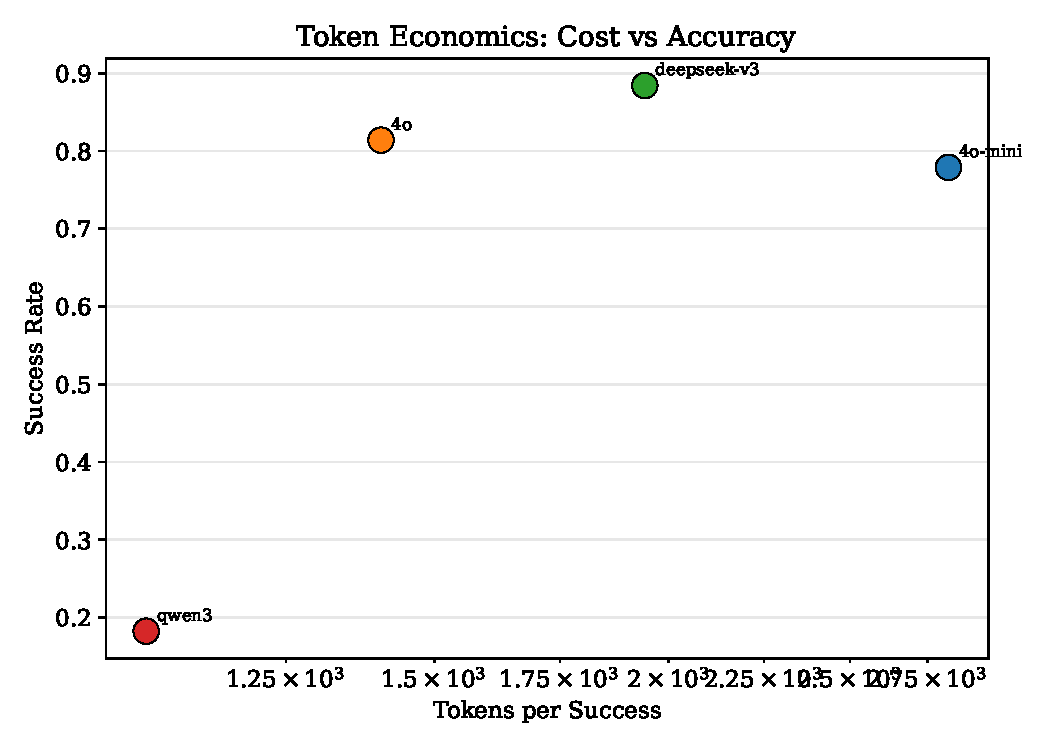
\includegraphics[width=0.7\linewidth]{figures/token_economics.pdf}
\caption{Token economics: tokens per success vs.\ success rate. DeepSeek-V3 dominates on both cost and accuracy.}
\label{fig:token}
\end{figure}

\FloatBarrier
